\documentclass[../../main/main.tex]{subfiles}
\graphicspath{{./figures/}}

\dominitoc
\faketableofcontents

\makeatletter
\renewcommand{\@chapapp}{Chimie -- chapitre}
\makeatother

% \toggletrue{student}
\HideSolutionstrue
\toggletrue{corrige}
% \renewcommand{\mycol}{black}
\renewcommand{\mycol}{gray}

\begin{document}
\setcounter{chapter}{1}

\chapter{Transformation et \'equilibre chimique}

\vfill

\begin{prgm}
	\begin{tcb}*(ror)"know"{Savoirs}
		\begin{itemize}[label=$\diamond$, leftmargin=10pt]
			\item Décrire qualitativement et quantitativement un
			      système chimique dans l'état initial ou dans un état d'avancement
			      quelconque.
			\item Exprimer l'activité d'une espèce chimique pure ou
			      dans un mélange dans le cas de solutions aqueuses très diluées ou de
			      mélanges de gaz parfaits avec référence à l'état standard.
			\item Exprimer le quotient réactionnel.
			\item Identifier un état d'équilibre chimique.
		\end{itemize}
	\end{tcb}

	\begin{tcb}*(ror)"how"{Savoir-faire}
		\begin{itemize}[label=$\diamond$, leftmargin=10pt]
			\item Déterminer une constante d'équilibre.
			\item Prévoir le sens de l'évolution spontanée d'un système chimique.
			\item Déterminer la composition chimique du système dans l'état final, en
			      distinguant les cas d'équilibre chimique ou de transformation totale,
			      pour une transformation modélisée par une réaction chimique unique.
		\end{itemize}
	\end{tcb}
\end{prgm}

\vfill
\minitoc
\vfill

\newpage

\section{Avancement d'une réaction}
\subsection{Présentation}
On considère la réaction de combustion du méthane~:
\csw{
	\[
		\ce{CH4\gaz{} + 2 O2\gaz{} = CO2\gaz{} + 2H2O\gaz}
	\]
}\vspace{-15pt}

Lorsqu'\textbf{une} molécule de méthane réagit, \textbf{deux} molécules de
dioxygène sont consommées et il se créé \textbf{une} molécule de dioxyde de
carbone et \textbf{une} d'eau. Cette réaction part de conditions initiales et
avance dans le temps, jusqu'à ce qu'elle s'arrête. Pour rendre compte de cette
évolution, on introduit une grandeur~: l'\textbf{avancement molaire}.

\begin{tcb}[label=def:xi, sidebyside, righthand ratio=.3](defi){Avancement molaire}
	\csw{
		La grandeur $\xi$ est appelée \textbf{avancement molaire de la réaction}, et
		elle permet de suivre l'évolution des quantités de matière des réactifs et
		des produis au cours d'une transformation chimique.
	}
	\tcblower
	\tcbsubtitle{\fatbox{Unités}}
	\csw{
		$\xi$ est homogène à une quantité de matière et s'exprime en mol.
	}
\end{tcb}

Ainsi, quand $\xi$ (se prononce «~ksi~») moles de
$\ce{CH4}$ réagissent, $2\xi$ moles de O$_2$ sont consommées pour augmenter de
$\xi$ moles la quantité de matière de CO$_2$ et de $2\xi$ moles celle de l'eau.

On détermine cet avancement grâce à un \textbf{tableau d'avancement}~:

\begin{tcb}[label=def:tabav](defi){Tableau d'avancement}
	Le \textbf{tableau d'avancement} est l'outil central pour étudier une
	réaction chimique. Il est composé de 3 ou 4 lignes, comprenant
	\begin{enumerate}
		\item \csw{
			      L'équation bilan, équilibrée grâce aux nombres stœchiométriques~;
		      }
		\item \csw{
			      L'état initial de la réaction avec les quantités de matière des
			      éléments~;
		      }
		\item \csw{
			      L'état en cours de réaction avec l'évolution des $n$ déduite des
			      nombres stœchiométriques~;
		      }
		\item \csw{
			      L'état final de la réaction avec les quantités de matières à
			      l'instant final.
		      }
	\end{enumerate}
	\begin{center}
		\def\rhgt{0.35}
		\centering
		\begin{tabularx}{\linewidth}{|l|c|YdYdYdY|}
			\hline
			\multicolumn{2}{|c|}{
				$\xmathstrut{\rhgt}$
			\textbf{Équation}}     &
			$a\ce{A}$              & $+$                 &
			$b\ce{B}$              & $\ra$               &
			$c\ce{C}$              & $+$                 &
			$d\ce{D}$                                      \\
			\hline
			$\xmathstrut{\rhgt}$
			\textit{État}          & \textit{Avance\mnt} &
			$n(\ce{A})$            & \vline              &
			$n(\ce{B})$            & \vline              &
			$n(\ce{C})$            & \vline              &
			$n(\ce{D})$                                    \\
			\hline
			$\xmathstrut{\rhgt}$
			Initial                & $\xi = 0$           &
			$n_0(\ce{A})$          & \vline              &
			$n_0(\ce{B})$          & \vline              &
			$n_0(\ce{C})$          & \vline              &
			$n_0(\ce{D})$                                  \\
			\hline
			$\xmathstrut{\rhgt}$
			Interm.                & $\xi$               &
			$n_0(\ce{A}) - a\xi$   & \vline              &
			$n_0(\ce{B}) - b\xi$   & \vline              &
			$n_0(\ce{C}) + c\xi$   & \vline              &
			$n_0(\ce{D}) + d\xi$                           \\
			\hline
			$\xmathstrut{\rhgt}$
			Final                  & $\xi_f$             &
			$n_0(\ce{A}) - a\xi_f$ & \vline              &
			$n_0(\ce{B}) - b\xi_f$ & \vline              &
			$n_0(\ce{C}) + c\xi_f$ & \vline              &
			$n_0(\ce{D}) + d\xi_f$                         \\
			\hline
		\end{tabularx}
	\end{center}
\end{tcb}

Remplissez le tableau suivant pour la combustion du méthane~:
\begin{center}
	\def\rhgt{0.50}
	\centering
	\begin{tabularx}{\linewidth}{|l|c|YdYdYdY|}
		\hline
		\multicolumn{2}{|c|}{
			$\xmathstrut{\rhgt}$
		\textbf{Équation}}                 &
		$\ce{CH_4\gaz{}}$                  & $+$       &
		$2\ce{O_2\gaz{}}$                  & $\ra$     &
		$\ce{CO_2\gaz{}}$                  & $+$       &
		$2\ce{H_2O\gaz}$                                 \\
		\hline
		$\xmathstrut{\rhgt}$
		Initial                            & $\xi = 0$ &
		\csw{$n_0(\ce{CH_4\gaz{}})$}       & \vline    &
		\csw{$n_0(\ce{O_2\gaz{}})$}        & \vline    &
		\csw{$n_0(\ce{CO_2\gaz{}})$}       & \vline    &
		\csw{$n_0(\ce{H_2O\gaz})$}                       \\
		\hline
		$\xmathstrut{\rhgt}$
		Interm.                            & $\xi$     &
		\csw{$n_0(\ce{CH_4\gaz{}}) - \xi$} & \vline    &
		\csw{$n_0(\ce{O_2\gaz{}}) - 2\xi$} & \vline    &
		\csw{$n_0(\ce{CO_2\gaz{}}) + \xi$} & \vline    &
		\csw{$n_0(\ce{H_2O\gaz}) + 2\xi$}                \\
		\hline
	\end{tabularx}
\end{center}

Quand on travaille à volume fixe, il peut être utile de travailler directement
avec les concentrations, donc avec $c_i = n_i/V$ avec $V$ le volume. On peut
donc définir l'avancement volumique~:

\begin{tcb}[label=def:x, sidebyside, righthand ratio=.4](defi){Avancement volumique}
	On définit $x$ l'\textbf{avancement volumique} de la réaction, tel que
	\csw{
		\[
			\boxed{x = \frac{\xi}{V}}
		\]
	}
	\tcblower
	\tcbsubtitle{\fatbox{Unités}}
	\csw{
		$x$ est homogène à une concentration et s'exprime en $\si{mol.L^{-1}}$.
	}
\end{tcb}

\subsection{Coefficients stœchiométriques algébriques}

Comme il est maintenant d'usage de le faire, on peut généraliser l'écriture
d'une réaction en faisant passer tous les termes d'un même côté. Par exemple,
pour la combustion du méthane~:
\[
	\ce{0 = CO2\gaz{} + 2H2O\gaz{} - CH4\gaz{} - 2O2\gaz{}}
\]
Ceci fait apparaître les \textbf{coefficients stœchiométriques algébriques}, que
l'on note $\nu_i$ (se lit «~nu~»). Une équation bilan peut donc se mettre sous
la forme générale
\csw{
	\[
		\boxed{\sum_i \nu_i\mathrm{X}_i = 0}
	\]
}
avec $\mathrm{X}_i$ les espèces intervenant dans la réaction. On a donc $\nu_i
	>0$ si $\mathrm{X}_i$ est un produit, et $\nu_i < 0$ si c'est un réactif. Dans
l'exemple de la combustion du méthane, on a
\csw{
	\[
		\begin{array}{rcl}
			\nu_{\ce{CH4}} = -1 \qquad & \text{et} \qquad & \nu_{\ce{O2}}=-2 \\
			\nu_{\ce{CO2}} = 1 \qquad  & \text{et} \qquad & \nu_{\ce{H20}}=2
		\end{array}
	\]
}

On peut donc généraliser la quantité de matière d'un composant directement avec
les coefficients algébriques~:
\csw{
	\[
		\boxed{n(\ce{X_i}) = n_0(\ce{X_i}) + \nu_i\xi}
	\]
}
avec $n(\ce{X_i})$ la quantité de matière de l'élément $\ce{X_i}$,
$n_0(\ce{X_i})$ sa quantité initiale et $\xi$ l'avancement.

\begin{tcb}*(expe)<itc>"trans"{Transition}
	On peut trouver différents états finaux selon les propriétés des réactions
	et la composition initiale de celles-ci. Introduisons un peu de vocabulaire
	pour distinguer ces cas et les étudier.
\end{tcb}

\section{États d'équilibre et final d'un système chimique}
\subsection{Réactions totale et limitée}

\begin{tcb}[label=def:final, sidebyside](defi)
	{Avancements final et maximal, réactions totale et limitée}
	\tcbsubtitle{\fatbox{Final ou maximal}}
	\csw{
		À l'état final, \textbf{quel qu'il soit}, les quantités des matières sont
		données par l'\textbf{avancement final} $\xi_f$. L'avancement \xul{maximal}
		$\xi_{\max}$ est l'avancement obtenu quand au moins un des \xul{réactifs est
			épuisé}.
	}
	\tcblower
	\tcbsubtitle{\fatbox{Totale ou limitée}}
	\csw{
		Quand $\xi_f = \xi_{\max}$, la réaction et alors \textbf{totale}. Sinon,
		elle est \textbf{limitée}. Une réaction totale se note avec un signe
		$\rightarrow$.
	}
\end{tcb}

\subsubsection{Réaction totale}

Reprenons l'exemple initial, et déterminons l'avancement final en supposant que
l'on part avec
\[
	n_{\ce{CH4}}^0 = \SI{2}{mol} \qet n_{\ce{O2}}^0 = \SI{3}{mol}
\]
et que la réaction est totale.

\begin{tcb}(tool){Réactif limitant}
	Pour trouver quel réactif et limitant, on cherche quelle expression entre
	$n_{\ce{CH4}}^0-\xi_{\max} $ et $n_{\ce{O2}}^0-2\xi_{\max} $ donne \textbf{le
		plus petit $\mathbf{\xi_{\max}}$}.
	\begin{itemize}
		\item \csw{
			      si $\ce{CH4}$ est limitant, alors $\xi_{\max} = \SI{2}{mol}$~;
		      }
		\item \csw{
			      si $\ce{O2}$ est limitant, alors $\xi_{\max} = \SI{1.5}{mol}$.
		      }
	\end{itemize}
	C'est donc le \csw{\textbf{dioxygène}} qui est limitant, et l'avancement
	maximal est de \csw{\SI{1.5}{mol}}.
\end{tcb}
On complète alors le tableau d'avancement~:

\begin{center}
	\def\rhgt{0.50}
	\centering
	\begin{tabularx}{\linewidth}{|l|c|YdYdYdY|}
		\hline
		\multicolumn{2}{|c|}{
			$\xmathstrut{\rhgt}$
		\textbf{Équation}} &
		$\ce{CH_4\gaz{}}$  & $+$          &
		$2\ce{O_2\gaz{}}$  & $\ra$        &
		$\ce{CO_2\gaz{}}$  & $+$          &
		$2\ce{H_2O\gaz{}}$                  \\
		\hline
		$\xmathstrut{\rhgt}$
		Initial (\si{mol}) & $\xi = 0$    &
		\csw{$2$}          & \vline       &
		\csw{$3$}          & \vline       &
		\csw{$0$}          & \vline       &
		\csw{$0$}                           \\
		\hline
		$\xmathstrut{\rhgt}$
		Interm. (\si{mol}) & $\xi$        &
		\csw{$2 - \xi$}    & \vline       &
		\csw{$3 - 2\xi$}   & \vline       &
		\csw{$0 + \xi$}    & \vline       &
		\csw{$0 + 2\xi$}                    \\
		\hline
		$\xmathstrut{\rhgt}$
		Final (\si{mol})   & $\xi_{\max}$ &
		\csw{$\num{0.5}$}  & \vline       &
		\csw{$\num{0}$}    & \vline       &
		\csw{$\num{1.5}$}  & \vline       &
		\csw{$\num{3}$}                     \\
		\hline
	\end{tabularx}
\end{center}

Il existe des situations où \textbf{tous les réactifs} sont limitant,
c'est-à-dire que l'avancement maximal met à $0$ toutes les quantités de matière
dans l'état final. On dit alors que les réactifs ont été introduits en
\textbf{proportions stœchiométriques}~:

\begin{tcbraster}[raster columns=2, raster equal height=rows]
	\begin{tcb}[label=def:propsto, cnt, bld](defi){Proportions stœchiométriques}
		\csw{
			On dit que les réactifs ont été introduits dans des proportions
			stoechiométriques si les quantités de matière de tous les réactifs
			s'annulent si l'avancement était maximal.
		}
	\end{tcb}
	\begin{tcb}(prop)'r'{Proportions stœchiométriques}
		Si c'est le cas, alors les réactifs vérifient
		\csw{
			\begin{gather*}
				\boxed{\frac{n_0(\ce{A})}{a} = \frac{n_0(\ce{B})}{b} = \xi_{\max}}
				\\\Lra
				n_0(\ce{B}) = \frac{b}{a} \ce{A}
			\end{gather*}
		}
		\vspace{-15pt}
	\end{tcb}
\end{tcbraster}

\begin{tcb}(tool){Réactions totales}
	Pour répondre à un exercice avec une réaction totale~:
	\begin{enumerate}
		\item \csw{
			      Dresser le tableau d'avancement~;
		      }
		\item \csw{
			      Écrire et équilibrer la réaction~;
		      }
		\item \csw{
			      Déterminer les quantités initiales des réactifs~;
		      }
		\item \csw{
			      Déterminer l'avancement maximal~;
		      }
		\item \csw{
			      Conclure.
		      }
	\end{enumerate}
\end{tcb}

\begin{tcb}[width=\linewidth, breakable](appl){Exercice}
	Lorsque l'on met du zinc solide dans un solution d'acide chlorhydrique, on
	observe un dégagement de dihydrogène et la formation d'ions zinc
	\ce{Zn^{2+}}.
	\smallbreak
	Le système initial est composé de $\SI{0.11}{g}$ de zinc et
	d'une solution de \SI{20}{mL} d'acide chlorhydrique à $\SI{5.0}{mol.L^{-1}}$.
	\smallbreak
	\textbf{Déterminer le volume de dihydrogène formé}.
	\smallbreak
	Le volume molaire des gaz est $\SI{24.5}{L.mol^{-1}}$, et la masse molaire du
	zinc est $M(\ce{Zn}) = \SI{65.38}{g.mol^{-1}}$.
	\tcblower
	\csw{
	On traduit l'énoncé avec l'équation
	\[
		\boxed{\ce{Zn\sol{} + 2H+\aqu \rightarrow Zn^{2+}\aqu{} + H2\gaz{} }}
	\]
	Les quantités initiales de réactifs sont
	\[
		\boxed{n_{\ce{Zn}}^0 = \frac{m}{M(\ce{Zn})} = \SI{1.68e-3}{mol}}
		\qet
		\boxed{n_{\ce{H+}}^0 = [\ce{H+}]V = \SI{1.00e-1}{mol}}
	\]
	}
	\begin{center}
		\def\rhgt{0.50}
		\centering
		\begin{tabularx}{\linewidth}{|l|c|YdYdYdY|}
			\hline
			\multicolumn{2}{|c|}{
				$\xmathstrut{\rhgt}$
			\textbf{Équation}}         &
			\csw{$\ce{Zn\sol}$}        & $+$          &
			\csw{$\ce{2H+\aqu}$}       & $\ra$        &
			\csw{$\ce{Zn^{2+}\aqu{}}$} & $+$          &
			\csw{$\ce{H2\gaz{}}$}                       \\
			\hline
			$\xmathstrut{\rhgt}$
			Initial (\si{mmol})        & $\xi = 0$    &
			\csw{$\num{1.68}$}         & \vline       &
			\csw{$\num{100}$}          & \vline       &
			\csw{$\num{0}$}            & \vline       &
			\csw{$\num{0}$}                             \\
			\hline
			$\xmathstrut{\rhgt}$
			Interm. (\si{mmol})        & $\xi$        &
			\csw{$\num{1.68} -\xi$}    & \vline       &
			\csw{$\num{100} -2\xi$}    & \vline       &
			\csw{$\xi$}                & \vline       &
			\csw{$\xi$}                                 \\
			\hline
			$\xmathstrut{\rhgt}$
			Final (\si{mmol})          & $\xi_{\max}$ &
			\csw{$\num{0}$}            & \vline       &
			\csw{$\num{96.64}$}        & \vline       &
			\csw{$\num{1.68}$}         & \vline       &
			\csw{$\num{1.68}$}                          \\
			\hline
		\end{tabularx}
	\end{center}
	\csw{
		On trouve l'avancement maximal $\xi_{\max} = \SI{1.68e-3}{mol}$, et on
		obtient le volume de $\ce{H2\gaz{}}$ avec son volume molaire
		\[\boxed{V_{\ce{H2}} = n_{\ce{H2}}V_m = \SI{41}{mL}}\]
	}
\end{tcb}

\subsubsection{Réaction limitée}

Une transformation limitée veut dire qu'il reste \textbf{toujours un peu de
	réactif et un peu de produit}. Ceci est possible puisqu'il peut se produire la
réaction
\begin{center}
	réactifs $\longrightarrow$ produits
\end{center}
mais dès que les produits sont présents, il peut aussi se passer
\begin{center}
	réactifs $\longleftarrow$ produits
\end{center}
On dit alors qu'il y a \textbf{équilibre chimique} lorsque les \textbf{deux
	réactions ont des actions inverses l'une de l'autre}. On voit donc les écritures
suivantes~:
\[
	\csw{
		\boxed{
			\ce{\alpha_1R_1 + \alpha_2R_2} +…
			\xrightleftharpoons[\rm indirect]{\rm direct}
			\ce{\beta_1P_1 +\beta_2P_2} +…
		}
	}
	\qou
	\csw{
		\boxed{
			\ce{\alpha_1R_1 + \alpha_2R_2} +…
			=
			\ce{\beta_1P_1 +\beta_2P_2}+…
		}
	}
\]

\subsection{Quantifications de l'avancement}

Il y a d'autres grandeurs utilisées pour décrire l'avancement~:

\begin{tcb}[label=def:tauxconvdissrendement, tabularx={Y|Y|Y}](defi)
	{Taux de conversion, coefficient de dissociation et rendement}
	\textbf{Taux de conversion} &
	\textbf{Coefficient de dissociation} &
	\textbf{Rendement}\\\hline
	On définit le taux de conversion d'un réactif X$_i$ comme
	\csw{
		\[
			\boxed{
				\tau(t) = \frac{n_{\ce{X_i}}^0 - n_{\ce{X_i}}(t)}{n_{\ce{X_i}}^0}
			}
		\]
	}
	Il vaut 0 à $t=0$, et 1 s'il a complètement été consommé. &
	Le coefficient de dissociation $\alpha$ est le taux de conversion dans le
	cas où \textbf{seul un réactif} se dissocie. &
	Le rendement est le rapport entre l'avancement à un instant $t$ et
	l'avancement \textit{maximal} $\xi_{\max}$. On a
	\csw{
		\[
			\boxed{\eta = \frac{\xi}{\xi_{\max}}}
		\]
	}

\end{tcb}

\begin{tcb}*(expe)<itc>"trans"{Transition}
	Nous cherchons donc un moyen de mettre en place des grandeurs pour
	déterminer le sens d'évolution d'un système en décrivant les actions des
	deux sens de la réaction.
\end{tcb}

\subsection{Quotient de réaction}

Pendant une réaction chimique, réactifs et produits s'opposent dans leur action
vis-à-vis de l'évolution du système.
Pour quantifier la tendance évolutive du l'équation, on fait appel aux
\textbf{activités} des éléments mis en jeu, \textit{via} une grandeur appelée
\textbf{quotient de réaction}.

\begin{tcb}[label=quoreac](defi){Quotient de réaction}
	Soit une réaction
	\[\ce{\alpha_1R_1 + \alpha_2R_2} +…
		=
		\ce{\beta_1P_1 +\beta_2P_2}+…\]
	qui peut également s'écrire
	\[ \sum_i \nu_i\mathrm{X}_i = 0\]
	Le quotient de réaction $Q_r$ est alors
	\csw{
		\[
			\boxed{Q_r = \frac{a(\ce{P_1})^{\beta_1} \times
					a(\ce{P_2})^{\beta_2} \times…}{
					a(\ce{R_1})^{\alpha_1} \times
					a(\ce{R_2})^{\alpha_2} \times…}}
			\qou
			\boxed{Q_r = \prod_i a(\ce{X_i})^{\nu_i}}
		\]
	}
\end{tcb}

\begin{tcb}[label=exem:qr, sidebyside, righthand ratio=.45](appl){Exemples}
	Écrire les quotients de~:
	\begin{enumerate}
		\item $\ce{2I^-\aqu{} + S2O8^{2-}\aqu{} = I2\aqu{} +2SO4^{2-}\aqu}$
		\item $\ce{Ag+\aqu{} + Cl^-\aqu{} = AgCl\sol}$
		\item $\ce{2FeCl3\gaz{} = Fe2Cl6\gaz{}}$
	\end{enumerate}
	\tcblower
	\vspace{+15pt}
	\begin{enumerate}
		\mitem
		\csw{
			\[
				Q_r = \frac{
					[\ce{I2}]\times[\ce{SO4^{2-}}]^2
				}{
					[\ce{I-}]^2\times [\ce{S2O8^{2-}}]
				}
			\]
		}
		\mitem
		\csw{
			\[
				Q_r =
				\frac{c\degree^2
				}{
					[\ce{Ag+}]\times[\ce{Cl-}]
				}
			\]
		}
		\mitem
		\csw{
			\[
				Q_r = \frac{P_{\ce{Fe2Cl6}}/P\degree
				}{
					P_{\ce{FeCl3}}{}^2/P\degree{}^2}
				=
				P\degree\frac{P_{\ce{Fe2Cl6}}
				}{
					P_{\ce{FeCl3}}{}^2
				}
			\]
		}
	\end{enumerate}
	\vspace{-15pt}
\end{tcb}

\subsection{Constante d'équilibre}
À l'équilibre chimique, les produits et réactifs se combinent dans des sens
opposés tout à fait équilibrés. On définit donc la constante d'équilibre~:

\begin{tcb}[label=def:K](defi){Constante d'équilibre}
	À toute réaction chimique est associée une grandeura appelée \textbf{constante
		d'équilibre}, notée $K\degree$, qui ne dépend \textbf{que de la réaction
		considérée et de la température}. Elle est égale au quotient réactionnel à
	l'équilibre chimique (état final)~:
	\csw{
		\[
			\boxed{K \degree = Q_{r, \eq}}
		\]
	}
	On l'appelle aussi la \textbf{relation de Guldberg-Waage} ou \textbf{loi
		d'action des masses}.
\end{tcb}

Le quotient de réaction va évoluer de telle sorte à être égal à la constante de
réaction à l'équilibre~: celle-ci permet de déterminer l'état d'équilibre du
système, puisqu'elle donnera le lien entre les activités des composants à
l'avancement final et donc la composition du système.

On constate assez évidemment que la constante d'équilibre d'une réaction écrit
dans un sens est l'\textbf{inverse} de la constante d'équilibre de la même
réaction écrite dans l'autre sens.

\begin{tcb}[width=\linewidth, breakable](appl){Exercice}
	Soit la réaction de l'acide éthanoïque avec l'eau~:
	\[\ce{CH3COOH\aqu{} + H2O\liq{} = CH3COO^{-}\aqu{} + H3O^{+}\aqu{}}\]
	de constante $K \degree = \num{1.78e-5}$. On introduit $c =
		\SI{1.0e-1}{mol.L^{-1}}$ d'acide éthanoïque et on note $V$ le volume de
	solution. Déterminer la composition à l'état final.
	\tcblower
	\begin{center}
		\def\rhgt{0.50}
		\centering
		\begin{tabularx}{\linewidth}{|l|c|YdYdYdY|}
			\hline
			\multicolumn{2}{|c|}{
				$\xmathstrut{\rhgt}$
			\textbf{Équation}}       &
			$\ce{CH_3COOH\aqu{}}$    & $+$       &
			$\ce{H2O\liq{}}$         & $\ra$     &
			$\ce{CH_3COO^{-}\aqu{}}$ & $+$       &
			$\ce{H_3O+\aqu{}}$                     \\
			\hline
			$\xmathstrut{\rhgt}$
			Initial                  & $x = 0$   &
			\csw{$c$}                & \vline    &
			\csw{excès}              & \vline    &
			\csw{$0$}                & \vline    &
			\csw{$0$}                              \\
			\hline
			$\xmathstrut{\rhgt}$
			Interm.                  & $x$       &
			\csw{$c - x$}            & \vline    &
			\csw{excès}              & \vline    &
			\csw{$x$}                & \vline    &
			\csw{$x$}                              \\
			\hline
			$\xmathstrut{\rhgt}$
			Final                    & $x = x_f$ &
			\csw{$c - x_f$}          & \vline    &
			\csw{excès}              & \vline    &
			\csw{$\xi_f$}            & \vline    &
			\csw{$\xi_f$}                          \\
			\hline
		\end{tabularx}
	\end{center}
	\csw{
		Par définition,
		\begin{gather*}
			K\degree =
			\frac{[\ce{H3O^{+}}]_f \times [\ce{CH3COO^{-}}]_f}
			{c\degree[\ce{CH3COOH}]_f}
			=
			\frac{x_f{}^2}{c\degree(c-x_f)}\\
			\Leftrightarrow
			x_f{}^2 + K\degree c\degree x_f - cK\degree c\degree = 0
		\end{gather*}
		On simplifie les calculs en ignorant $c\degree = \SI{1}{mol.L^{-1}}$. Ainsi
		ce polynôme a deux racines~:
		\begin{gather*}
			x_{f,1} = \frac{-K\degree - \sqrt{K\degree^2+4K\degree c}}{2}
			\qet
			x_{f,2} = \frac{-K\degree + \sqrt{K\degree^2+4K\degree c}}{2}\\
			x_{f,1} = \SI{-1.34e-3}{mol.L^{-1}}
			\qet
			x_{f,2} = \SI{1.32e-3}{mol.L^{-1}}
		\end{gather*}
		dont seule la seconde fait sens, étant donné qu'il n'y a pas de produit au
		départ~: on garde donc
		\[\xul{x_f = \SI{1.32e-3}{mol.L^{-1}}}\]
	}

\end{tcb}

Dans cet exemple, on pouvait effectuer une simplification en considérant la
valeur de la constante d'équilibre. En effet, le fait que la constante
d'équilibre soit petite veut dire l'équilibre va être atteint très vite, dès
qu'un peu des produits sont formés et que le ratio de leurs activités sur celles
des réactifs est égal à la constante d'équilibre. On a donc les propriétés
suivantes sur la constante d'équilibre~:

\begin{tcb}[label=prop:K](ror){Constante d'équilibre et avancement}
	De manière qualitative, on a~:
	\begin{itemize}
		\item \csw{
			      si $K < 1$, la réaction est favorisée dans le sens $\leftarrow$,
			      et si $K < \num{e-4}$, alors la réaction est \textbf{peu avancée}
			      dans le sens $\rightarrow$~;
		      }
		\item \csw{
			      si $K > 1$, alors la réaction est favorisée dans le sens
			      $\rightarrow$, et si $K > \num{e4}$, alors la réaction est
			      \textbf{totale} (ou quasi-totale) dans le sens $\rightarrow$.
		      }
	\end{itemize}
\end{tcb}

Ainsi, dans l'exercice précédent, on sait que $x \ll c$ puisque $K \ll
	\num{e-4}$~: on peut donc écrire
\csw{
\[
	K = \frac{x_f{}^2}{c}
	\Lra
	x_f = \sqrt{Kc} = \SI{1.33e-3}{mol.L^{-1}}
\]
}

\begin{tcb}*(expe)<itc>"trans"{Transition}
	Comment la connaissance de l'équilibre d'un système peut-elle alors nous
	permettre de prédire son avancée~?
\end{tcb}

\section{Évolution d'un système chimique}
\subsection{Quotient réactionnel et sens d'évolution}

Étant donné que la constante d'équilibre est égale au quotient réactionnel à
l'équilibre, les activités des éléments chimiques vont évoluer de telle sorte à
ce que le quotient réactionnel atteigne l'équilibre~: s'il est inférieur à
$K\degree$ au départ, il doit augmenter au cours de la réaction et donc
augmenter les produits et réduire les réactifs, et inversement. On retiendra

\begin{tcb}[label=prop:qrsensevo](prop){Sens d'évolution d'un système}
	\begin{itemize}
		\item \csw{
			      Si $Q_r < K$, la réaction se déroule dans le sens direct~;
		      }
		\item \csw{
			      Si $Q_r > K$, la réaction se déroule dans le sens indirect~;
		      }
	\end{itemize}
	\begin{center}
		\sswitch{
			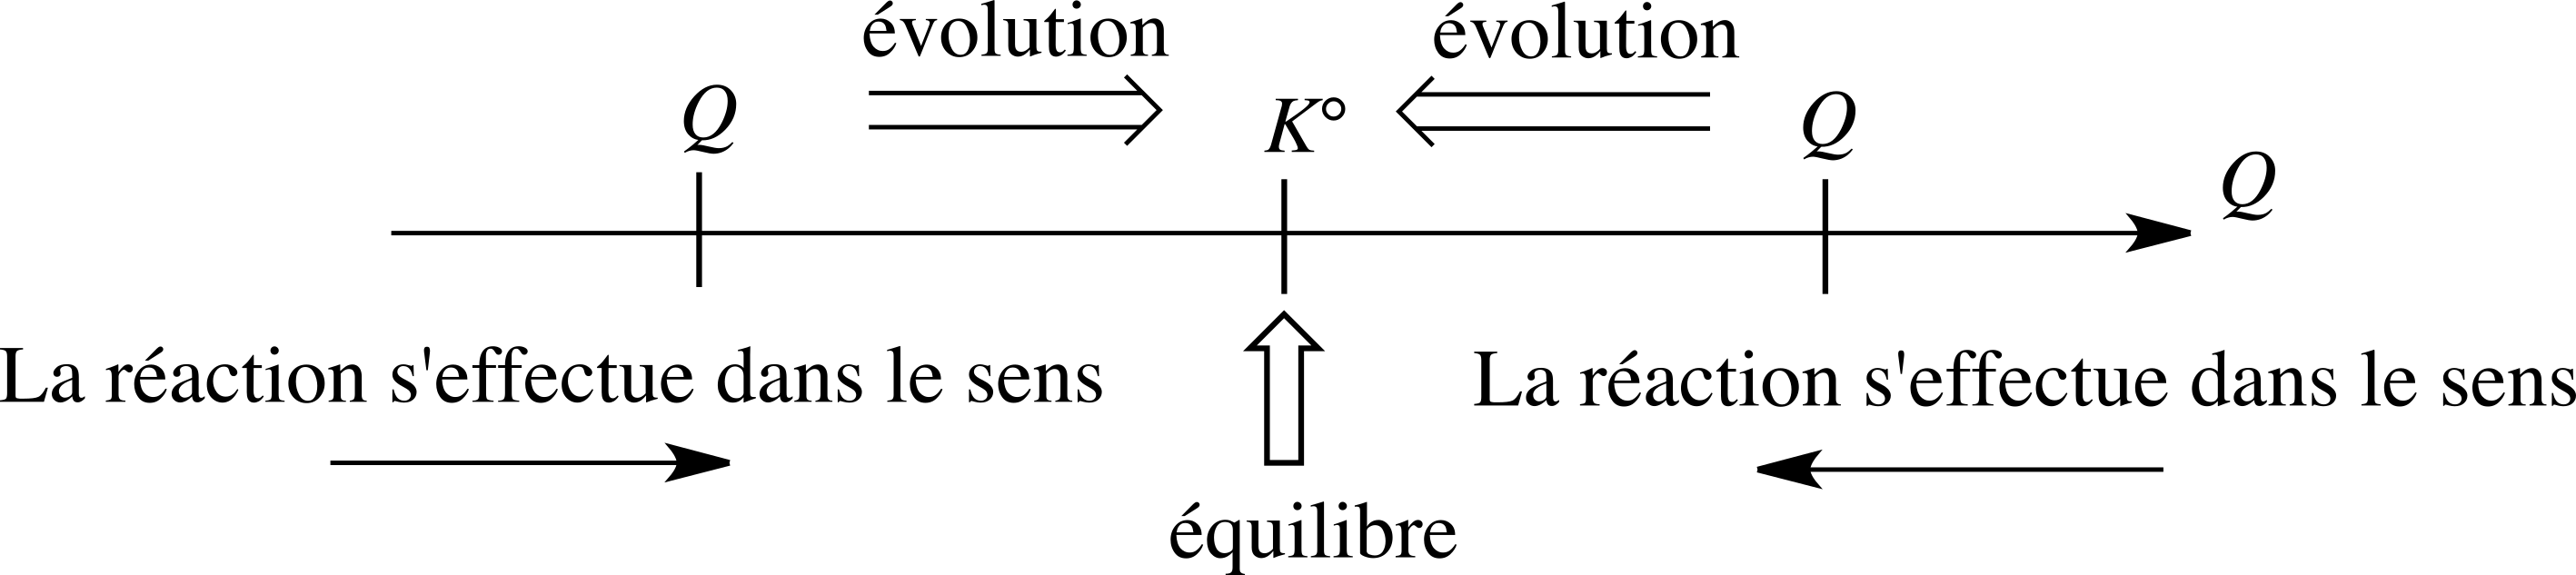
\includegraphics[width=.7\linewidth, draft=true]{sensevo}
		}{
			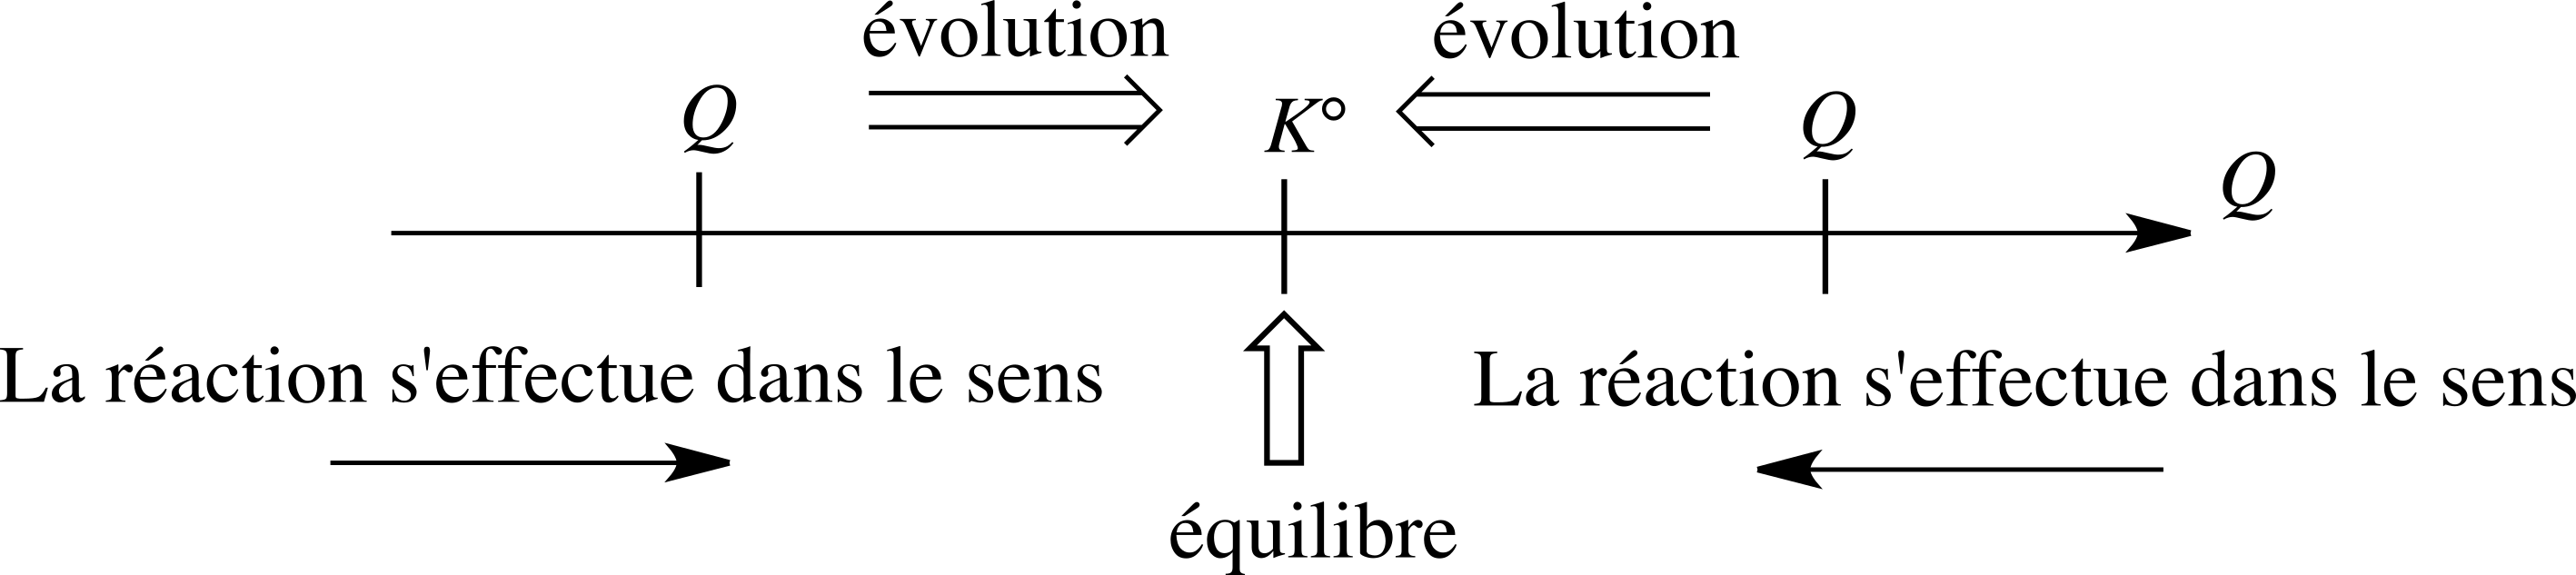
\includegraphics[width=.7\linewidth]{sensevo}
		}
		\captionof{figure}{}
	\end{center}
\end{tcb}

Prenons par exemple la réaction

\centersright{%
	$\ce{Ag^{+}\aqu{} + Cl^{-}\aqu{} = AgCl\sol{}}$%
}{%
	$K\degree = \num{e9.7}$%
}

\begin{enumerate}
	\item Si $[\ce{Ag^{+}}]_i = [\ce{Cl-}]_i = \SI{e-3}{mol.L^{-1}}$, alors
	      \csw{
		      \[
			      Q_{r,0} = \frac{c\degree^2}{[\ce{Ag^{+}}]_i \times [\ce{Cl-}]_i}
			      = \num{e6} < K\degree
		      \]
	      }
	      et la réaction se passe dans le sens \csw{direct~: on forme du précipité.}
	\item Si $[\ce{Ag^{+}}]_i = [\ce{Cl-}]_i = \SI{e-6}{mol.L^{-1}}$, alors
	      \csw{
		      \[
			      Q_{r,0} = \frac{c\degree^2}{[\ce{Ag^{+}}]_i \times [\ce{Cl-}]_i}
			      = \num{e12} > K\degree
		      \]
	      }
	      et la réaction se passe dans le sens \csw{indirect~: on dissout le précipité.}
\end{enumerate}

\begin{tcb}[width=\linewidth, breakable](appl){Exercice}
	Soit la synthèse de l'ammoniac~:

	\centersright{$\ce{N2\gaz{} + 3H2\gaz{} = 2NH3\gaz{}}$}{$K\degree = \num{0.5}$}

	On introduit \SI{3}{mol} de diazote, \SI{5}{mol} de dihydrogène et
	\SI{2}{mol} d'ammoniac sous une pression de \SI{200}{bars}.
	\begin{enumerate}
		\item Déterminer les pressions partielles des gaz.
		\item Dans quel sens se produit la réaction~?
	\end{enumerate}
	\tcblower
	\begin{enumerate}
		\item
		      \csw{
			      Pour déterminer les pressions partielles, il nous faut la quantité
			      de matière totale de gaz~: $n_{\rm tot} = 2+3+5 = \SI{10}{mol}$. On
			      a donc
			      \[
				      p_{\ce{N2}} = x_{\ce{N2}}P = \SI{60}{bar}
				      \qquad
				      p_{\ce{H2}} = x_{\ce{H2}}P = \SI{100}{bar}
				      \qquad
				      p_{\ce{NH3}} = x_{\ce{NH3}}P = \SI{40}{bar}
			      \]
		      }
		      \vspace{-15pt}
		\item
		      \csw{
			      Pour connaître le sens de réaction, il faut le quotient
			      réactionnel~:
			      \[Q_{r,0} = \frac{p_{\ce{NH3}}{}^2\times p\degree^2}
				      {p_{\ce{N2}}\times p_{\ce{H2}}{}^3} = \num{2.7e-5}
			      \]
			      Comme $Q_{r,0} < K$, la réaction se produit dans le sens
			      \textbf{direct}~: on consomme $\ce{N2}$ et $\ce{H2}$ et on produit
			      $\ce{NH3}$.
		      }
	\end{enumerate}
\end{tcb}

\begin{tcb}*[label=ror:gaz](prop)"bomb"{Tableau avancement et gaz}
	On remarque que pour déterminer l'avancement d'une réaction avec des gaz, il
	faut avoir à tout instant la \textbf{quantité de matière totale de gaz} pour
	calculer les pressions partielles nécessaires au calcul de l'activité de
	chacun des gaz~: c'est pourquoi il est d'usage d'\textbf{ajouter une colonne
		$n_{\rm tot, gaz}$ dans les tableaux d'avancement}.
\end{tcb}

Dans le cas de l'exercice précédent, on ferait donc~:

\begin{center}
	\def\rhgt{0.50}
	\centering
	\begin{tabularx}{\linewidth}{|l|c|YdYdYdY|}
		\hline
		\multicolumn{2}{|c|}{
			$\xmathstrut{\rhgt}$
		\textbf{Équation}}  &
		$\ce{N_2\gaz{}}$    & $+$       &
		$3\ce{H_2\gaz{}}$   & $=$       &
		$2\ce{NH_3\gaz{}}$  & \vline    &
		$n_{\tot, gaz}$                   \\
		\hline
		$\xmathstrut{\rhgt}$
		Initial (\si{mol})  & $\xi = 0$ &
		\csw{$3$}           & \vline    &
		\csw{$5$}           & \vline    &
		\csw{$2$}           & \vline    &
		\csw{$10$}                        \\
		\hline
		$\xmathstrut{\rhgt}$
		Interm.  (\si{mol}) & $\xi$     &
		\csw{$3 - \xi$}     & \vline    &
		\csw{$5 - 3\xi$}    & \vline    &
		\csw{$2 + 2\xi$}    & \vline    &
		\csw{$10 - 2\xi$}                 \\
		\hline
	\end{tabularx}
\end{center}

\subsection{Cas des ruptures d'équilibre}

Quand la réaction contient des \textbf{solides ou liquides purs}, les activités
ne peuvent pas évoluer, elles \textbf{restent égales à 1}. Dans ce cas, on peut
arriver à ce qu'on appelle une \textit{rupture d'équilibre}. Regardons la
réaction de dissolution du chlorure de sodium, de masse molaire $M(\ce{NaCl}) =
	\SI{58.44}{g.mol^{-1}}$~:

\centersright{%
	$\ce{NaCl\sol{} = Na^{+}\aqu{} + Cl^{-}\aqu{}}$%
}{%
	$K\degree=33$%
}

On introduit \SI{2.0}{g} de sel dans \SI{100}{mL} d'eau. Déterminons l'état
d'équilibre.
\bigbreak
\leftcenters{%
	On introduit%
}{%
	\csw{$\DS n = \frac{m}{M(\ce{NaCl})} = \SI{0.034}{mol}$}%
}

\begin{center}
	\def\rhgt{0.35}
	\centering
	\begin{tabularx}{\linewidth}{|l|c|YdYdY|}
		\hline
		\multicolumn{2}{|c|}{
			$\xmathstrut{\rhgt}$
		\textbf{Équation}} &
		$\ce{NaCl\sol{}}$  & $=$           &
		$\ce{Na+\aqu{}}$   & $+$           &
		$\ce{Cl^{-}\aqu{}}$                  \\
		\hline
		$\xmathstrut{\rhgt}$
		Initial            & $\xi = 0$     &
		$n$                & \vline        &
		$0$                & \vline        &
		$0$                                  \\
		\hline
		$\xmathstrut{\rhgt}$
		Final              & $\xi = \xi_f$ &
		$n - \xi_f$        & \vline        &
		$\xi_f$            & \vline        &
		$\xi_f$                              \\
		\hline
	\end{tabularx}
\end{center}

La constante d'équilibre est
\csw{
	\begin{gather*}
		K\degree =
		\frac{[\ce{Na+}]\times[\ce{Cl-}]}{c\degree^2} =
		\frac{1}{c\degree^2} \left(\frac{\xi_f}{V}\right)^2
		\Lra
		\boxed{\xi_f = Vc\degree\sqrt{K\degree} = \SI{0.57}{mol}}
	\end{gather*}
}

Or, l'avancement maximal théorique est $\xi_{\max} = \csw{\SI{0.034}{mol}} <
	\xi_f$~: on ne peut donc pas atteindre l'équilibre, le solide est
\textbf{dissout en totalité}. On appelle ça une \textbf{rupture d'équilibre}.

\subsection{Résumé}

\begin{center}
	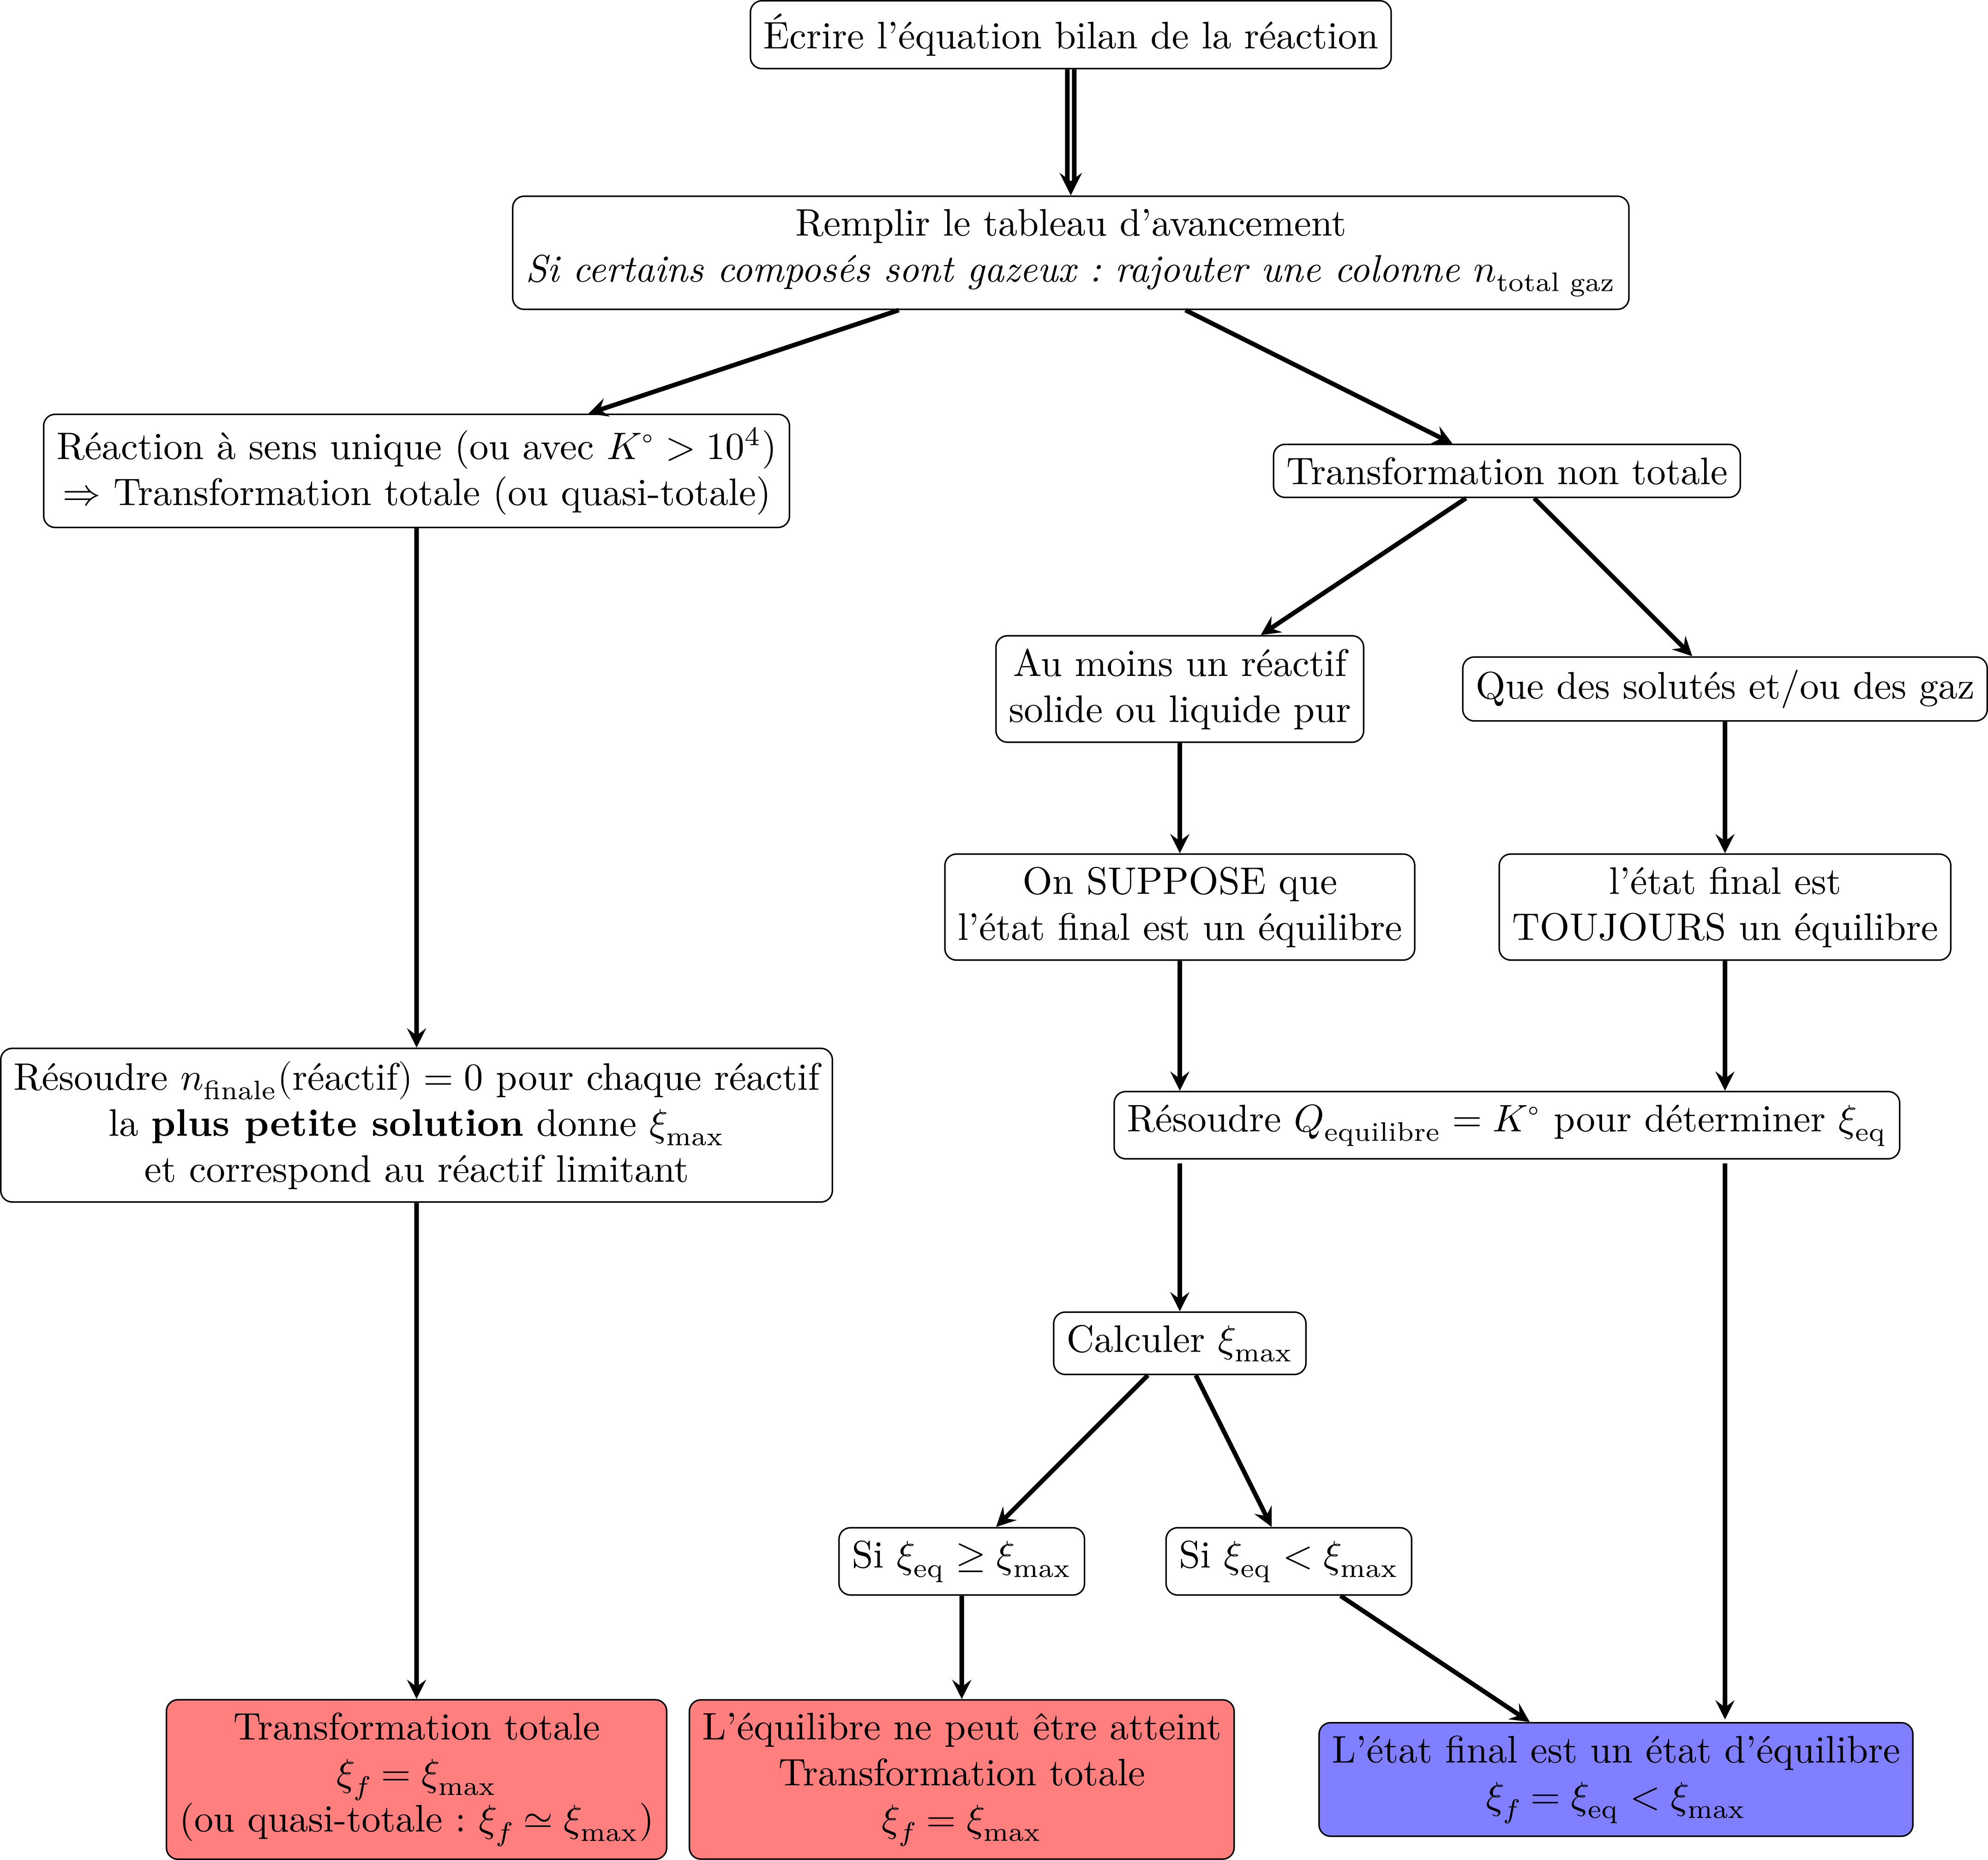
\includegraphics[width=\linewidth]{resume}
\end{center}
\end{document}
